\documentclass[pdf]{beamer}

\usepackage{amsmath}
\usepackage{amsfonts}
\usepackage{graphicx}

\mode<presentation>{}

\title{Extended Topic Models with Numerical Features}

\author{G\" okhan \c Capan, Ali Caner T\" urkmen}
\begin{document}
	
\begin{frame}
	\titlepage
\end{frame}

\begin{frame}{Introduction}
	
	\begin{itemize}
		\item Unsupervised learning, recover \emph{latent} topics in documents
		\item Can be thought of as clustering. Loosely equivalent to link prediction.
	\end{itemize}
	
\end{frame}

\begin{frame}{Latent Dirichlet Allocation}
	
	\begin{itemize}
		\item (Blei et al., 2003)
	\end{itemize}
	
\end{frame}

\begin{frame}{Comparison of Topic Models}
	
	\begin{itemize}
		%TODO: comparison slide from blei
		\item (Blei et al., 2003)
	\end{itemize}
	
\end{frame}

\begin{frame}{Coupled Topic Model Applications}
	
	\begin{itemize}
		\item Gokhan lit survey
	\end{itemize}
	
\end{frame}

\begin{frame}{LDA $\equiv$ Bayesian NMF up to parameterization }
	
	\begin{itemize}
		%TODO: comparison slide from blei
		\item (Jordan Blei) (Cemgil, 2009)
	\end{itemize}
	
\end{frame}



\begin{frame}{Coupled Matrix Factorization for Recovering Topics}
	
	\begin{figure}[h]
		\centering
		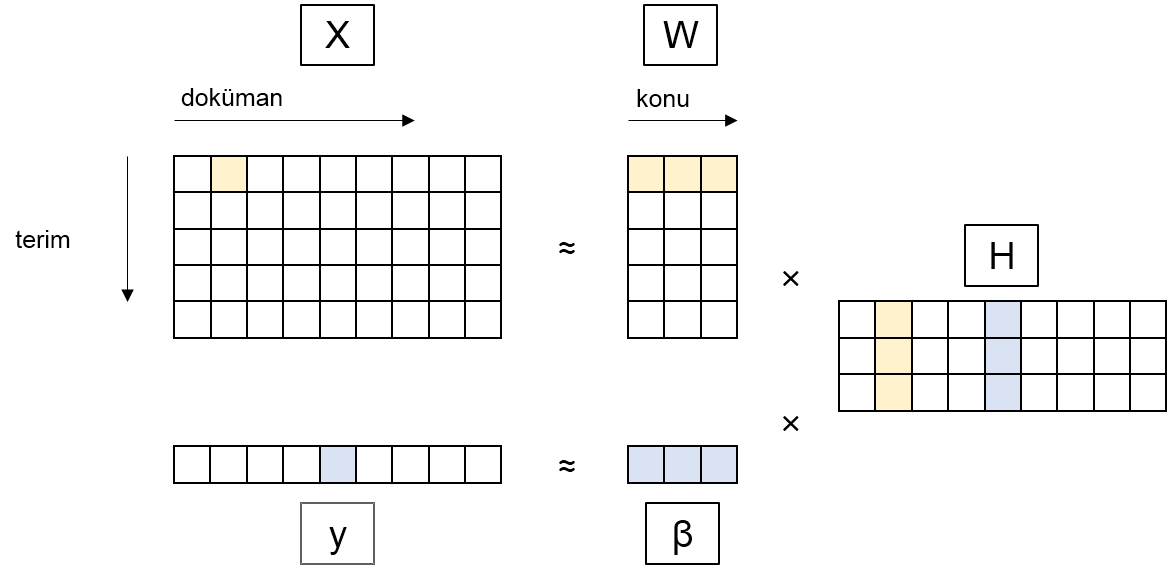
\includegraphics[width=9cm]{images/nmf2.png}
	\end{figure}
	
	\begin{itemize}
		
		\item Represent data with well-known algebraic structures
		\item Jointly guide topic assignments from multimodal datasets, in a probabilistically sound framework
		\item Easily extensible to semi-supervised learning, kernel methods
		\item (T. and Cemgil, 2016)
	\end{itemize}
	
\end{frame}

\begin{frame}{Extended Coupled NMF for Topic Learning with Count Features}
	
	\begin{figure}[h]
		\centering
		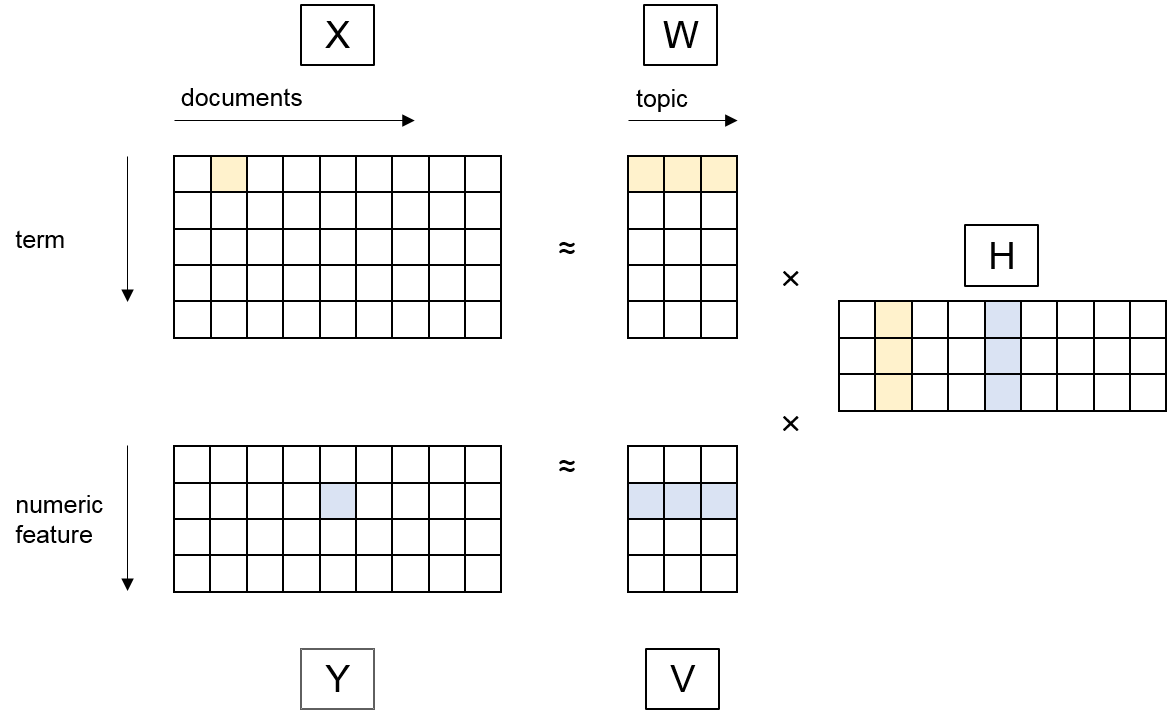
\includegraphics[width=7cm]{images/ext_nmf.png}
	\end{figure}
	
	\begin{itemize}
		\item $ y_{ij} | W, H \sim GPO(\sum_{t} w_{it} h_{tj}, \phi) $
		\item $ x_{kj} | V, H \sim GPO(\sum_{t} v_{kt} h_{tj}, \gamma) $
		\item Guide topic modeling with numeric count data
		\item Can assume priors $p(W), p(H), p(V)$ for Bayesian learning
	\end{itemize}
	
\end{frame}


\begin{frame}{Data Set and Features}
	
	\begin{itemize}
		\item {\bf Data Set:} News articles sampled from Anadolu Agency website. 1337 documents (can be expanded), ~3000 tokens after adjusting for document frequency. 
		\item {\bf Features:} Complexity features such as word count, sentence count, average sentence length, comma count. (TBD)
		\item {\bf Novel Features:} Etymological counts. Count the number of words from their etymological origins. Number of Arabic, Farsi, French words, etc. Source: TR Wiktionary Database Dump.
	\end{itemize}
	
\end{frame}

\begin{frame}{Learning}
	
	\begin{itemize}
		\item EM-like updates with multiplicative NMF update rules 
		\item Gibbs sampling assuming appropriate priors (tentative, out of scope for this project)
	\end{itemize}
	
\end{frame}

\begin{frame}{Conclusion}
	
	We propose two key contributions
	\begin{itemize}
		\item Put the topic modeling problem in a coupled NMF framework, extending with numerical features
		\item Use etymological counts for the Turkish language
	\end{itemize}
	
\end{frame}

\bibliography{zotero}{}
\bibliographystyle{apalike}
\end{document}